%; whizzy paragraph -pdf xpdf -latex ./whizzypdfptex.sh
%; whizzy-paragraph "^\\\\begin{frame}"
% latex beamer presentation.
% platex, latex-beamer でコンパイルすることを想定。 

%     Tokyo Debian Meeting resources
%     Copyright (C) 2009 Junichi Uekawa
%     Copyright (C) 2009 Nobuhiro Iwamatsu

%     This program is free software; you can redistribute it and/or modify
%     it under the terms of the GNU General Public License as published by
%     the Free Software Foundation; either version 2 of the License, or
%     (at your option) any later version.

%     This program is distributed in the hope that it will be useful,
%     but WITHOUT ANY WARRANTY; without even the implied warreanty of
%     MERCHANTABILITY or FITNESS FOR A PARTICULAR PURPOSE.  See the
%     GNU General Public License for more details.

%     You should have received a copy of the GNU General Public License
%     along with this program; if not, write to the Free Software
%     Foundation, Inc., 51 Franklin St, Fifth Floor, Boston, MA  02110-1301 USA

\documentclass[cjk,dvipdfmx,12pt]{beamer}
\usetheme{Tokyo}
\usepackage{monthlypresentation}

%  preview (shell-command (concat "evince " (replace-regexp-in-string "tex$" "pdf"(buffer-file-name)) "&")) 
%  presentation (shell-command (concat "xpdf -fullscreen " (replace-regexp-in-string "tex$" "pdf"(buffer-file-name)) "&"))
%  presentation (shell-command (concat "evince " (replace-regexp-in-string "tex$" "pdf"(buffer-file-name)) "&"))

%http://www.naney.org/diki/dk/hyperref.html
%日本語EUC系環境の時
\AtBeginDvi{\special{pdf:tounicode EUC-UCS2}}
%シフトJIS系環境の時
%\AtBeginDvi{\special{pdf:tounicode 90ms-RKSJ-UCS2}}

\title{東京エリアDebian勉強会}
\subtitle{第71回 2010年12月度}
\author{上川純一 dancer@debian.org\\IRC nick: dancerj}
\date{2010年12月18日}
\logo{
\includegraphics[width=8cm]{image200607/openlogo-light.eps}}

\begin{document}

\frame{\titlepage{}}

\section{}
\begin{frame}
 \frametitle{Agenda}
\begin{minipage}[t]{0.45\hsize}
  \begin{itemize}
  \item 注意事項
	\begin{itemize}
	 \item 飲食禁止
	 \item 宗教禁止
	 \item 営利活動禁止
	\end{itemize}
  \item 最近あったDebian関連のイベント報告
	\begin{itemize}
	 \item ??
	\end{itemize}
 \end{itemize}
\end{minipage} 
\begin{minipage}[t]{0.45\hsize}
 \begin{itemize}
  \item 2010年のDebian勉強会
  \item CACertの準備
  \item libsane
  \item Debian miniconf
  \item 2011 を妄想
 \end{itemize}
\end{minipage}
\end{frame}

\emtext{prework}

{\footnotesize
 \begin{prework}{ matsuu }

やったこと・おきたこと
\begin{itemize}
 \item Debian勉強会に参加するようになった。
 \item VPSでDebianを使い始めた。
 \item Debianのパッケージを参考にGentooパッケージを作った。
\end{itemize}
予想・やりたいこと
\begin{itemize}
 \item DebianとGentooは徐々に衰退していき、ALL YOUR DISTRIBUTION ARE
       BELONG TO CHROMEOS.
\end{itemize}
\end{prework}

\begin{prework}{ あらきやすひろ }

予想
\begin{itemize}
 \item 無事リリースされることによるDebian派生ディストロの大崩壊と回帰。
\end{itemize}
やりたいこと
\begin{itemize}
 \item Debianで仕事!
\end{itemize}
\end{prework}

\begin{prework}{ koedoyoshida }

やったこと
\begin{itemize}
 \item ddtssでレビュー(最近お休み中)
 \item 関西KOFでの関西Debianブースのお留守番
 \item 夏冬のイベントでの書籍の頒布
\end{itemize}
おきたこと
 \begin{itemize}
  \item Squeeze freeze
\end{itemize}
予想
\begin{itemize}
 \item  Squeeze release?
\end{itemize}
やりたいこと
\begin{itemize}
 \item 予定は未定
\end{itemize}
\end{prework}

\begin{prework}{ キタハラ }

やったこと
\begin{itemize}
\item 今年は一番何もしていない年ではないだろうか?ネットサーフィン用寝床PCも死んだままだし。
\end{itemize}
やりたいこと
\begin{itemize}
\item 来年はこれを復活し、あと会社にDebianマシンを復活させたいですね。
\end{itemize}
\end{prework}

\begin{prework}{ yamamoto }

やったこと
\begin{itemize}
 \item なんかポチポチと勝手に ppc64 ポートを、マズいラーメン屋の頑固オヤ
       ジのごとく、細く長く続けていた。
\end{itemize}
おきたこと
\begin{itemize}
 \item debian-ports に、sparc64 やら powerpcspe やら armhf やらがいきな
       り現れて、いっきに抜かれて行った。
\end{itemize}
予想
\begin{itemize}
 \item 次は arm64 かな?
\end{itemize}
やりたいこと
\begin{itemize}
 \item 頑固オヤジの迷惑なラーメンを、ひたすら生み出していく。
 \item arm64 ポートに参加できるといいな。
\end{itemize}
\end{prework}

\begin{prework}{ 本庄 }

やったこと
\begin{itemize}
\item 温泉行きました。
\end{itemize}
やりたいこと
\begin{itemize}
\item また行きたいです。
\end{itemize}
\end{prework}

\begin{prework}{ yyuu }

私事ではありますが、2009 年くらいから仕事で Debian を使えるようになりま
 した。2010 年はその環境の整備に費やしているうちにあっという間に過ぎてし
 まいました。

やったこと
\begin{itemize}
 \item lenny のシステムを 100 台以上の単位で扱うことができた
 \item 自分で個人的な apt のレポジトリを作って運用できるようになった
\end{itemize}
おきたこと
\begin{itemize}
 \item 特に思いつきませんでした...
\end{itemize}

予想
 \begin{itemize}
  \item squeeze がリリースされる (2010年?)
 \end{itemize}
やりたいこと
\begin{itemize}
 \item 一部の既存ホストを lenny から squeeze へ移行したい
 \item 新興プロジェクトの Debian パッケージ化にできるだけコミットしてい
       きたい。今年は Apache Thrift などにパッチを提供できたが、今後はも
       う少し手を広げたい
\end{itemize}
\end{prework}

\begin{prework}{ 野島 貴英 }

やったこと
\begin{itemize}
 \item debian-sidのKVM上でOpensolarisを稼働させた事。
 \item debian-sidの様々なソースコードいっぱい読んだこと。
       \footnote{\url{http://d.hatena.ne.jp/nozzy123nozzy/}}
\end{itemize}
予想
\begin{itemize}
\item いわゆる携帯型tabletPC等へdebian-sidを搭載するHackがそこいら中で起きる。
\end{itemize}
やりたいこと
\begin{itemize}
 \item Contribution \& Hack!Hack!Hack!(ソフトもハードも)
\end{itemize}
\end{prework}

\begin{prework}{ henrich }

やったこと
\begin{itemize}
 \item 5月: NMプロセスを進めてDDになった
 \item 7月: スイスからDebian傘買ってみた :)
 \item 8月: Debconf に参加した
 \item パッケージのアップデートを大体継続できた
 \item その他国内のイベントに参加した
 \item RC バグ潰しに参加した
 \item 多少ではあるが翻訳作業に参加した
 \item 手が付いていないことは以下
       \begin{itemize}
	\item netbeans のパッケージ
	\item eclipse-l10n のパッケージ(ソースを見つけられない…)
	\item Knoppix-Math を Debian ベースに誘う
	\item lenny インストール記事を JP ページに載せる
       \end{itemize}
\end{itemize}
やりたいこと
\begin{itemize}
 \item 開発者リファレンス訳の完了
 \item 初歩のプログラミングができるように(pythonあたり)
 \item debconf で何かしらの成果を出せるように事前準備
 \item l10n をもっと進められるようにもっとステップと成果を明確にしたい
\end{itemize}
\end{prework}

\begin{prework}{ 岩松 信洋 }

やったこと
\begin{itemize}
 \item 組み込み関係のサポート。
 \item SH4のemdebianサポート。
 \item Macbook 関係のサポート。
 \item DDになってからの始めてのリリース作業。
 \item Debconf への参加
\end{itemize}
おきたこと
\begin{itemize}
 \item Non-packaging contributors
 \item backports が正式サービスになった。 
 \item Squeeze フリーズ
 \item Miniconf が多く行われた。
 \item fjp の急逝
\end{itemize}
予想
\begin{itemize}
 \item Debian では SH4 unstable 入り
 \item 4G ネットワークがじわじわと浸透
 \item Android を使ったタブレットデバイス祭り
\end{itemize}
やりたいこと
\begin{itemize}
 \item web 系の開発
 \item 関数型言語の習得
\end{itemize}
\end{prework}

\begin{prework}{ 野首 }

2010年はほとんど何もしませんでした...
さすがにsqueezeは2011年にはリリースされていると思いたい。
\end{prework}

\begin{prework}{ まえだこうへい }

やったこと
\begin{itemize}
 \item Debian勉強会の運営(いつもどおり)
 \item 山田さんのJPへの勧誘・加入(よくやった)
 \item 他の勉強会での勧誘(Webアプリ開発者に交友関係は増えたがDebianへの
       直接的な成果はなし)
\end{itemize}
おきたこと(予想?)
\begin{itemize}
 \item SqueezeにはCouchDB 1.0.1が入らなさそう。
\end{itemize}
やりたいこと
\begin{itemize}
 \item いろいろpendingなものを再開する。
\end{itemize}
\end{prework}

\begin{prework}{ 上川純一 }

やったこと
\begin{itemize}
 \item 子供がうまれた、Debian活動レベルが低下した。
 \item 携帯電話はAndroid携帯電話がメインになって、パソコンをあまり起動し
       なくなった。
 \item 勉強会にくるようなメンバーで、Smart Phone (iPhone or Android)をもっ
       ていない人に出会わなくなってきた。
\end{itemize}
予想
\begin{itemize}
 \item さらなるスマートフォンとタブレットの普及とそれに伴うより自由で便
       利な環境への渇望。
 \item Debianとしてはその環境との相互運用性の向上と、そのデバイス自体で
       動くシステムとしてのすすみかたが二つ考えられる。
\end{itemize}
やりたいこと
\begin{itemize}
 \item 相互運用性は少なくとも向上したいと考えている。
\end{itemize}
\end{prework}


}

\emtext{イベント報告}

\emtext{2010年のふりかえり}

\begin{frame}{2010年の東京エリア}

 \begin{tabular}{|l|c|p{10em}|}
  \hline
  & 参加人数 & 内容\\
  \hline
  2010年1月 & 17 &  東京大学にて新年会 \\
  2010年2月 & 11 & Debian温泉,ocaml,haskell \\
  2010年3月 & 12 & weka,fftw,dpkg v3 quilt \\
  2010年4月 & 15 & upstart,piuparts,debtags \\
  2010年5月 & 22 & 筑波大学,kernel \\
  2010年6月 & 12 & OSC-Doリハーサル  \\
  2010年7月 & 0 & キャンセル(海)  \\
  2010年8月 & 3 & Debconf (NYC) \\
  2010年9月 & 30 & OSC Tokyo/Fall \\
  2010年10月 & 13 & 俺のDebianな一日 \\
  2010年11月 & 15 & ext4,btrfs,nilfs,ceph \\
  2010年12月 & 14 &  cacert, libsane \\
  \hline
 \end{tabular}
\end{frame}

\begin{frame}{2010年の関西}
  \begin{tabular}{|l|c|p{10em}|}
 \hline
 & 参加人数 & 内容 \\
 \hline
2010年1月 & 16 & Xen, 2010年企画 \\
2010年2月 & 16 & レンタルサーバでの利用, GAE \\
2010年3月 & 30? & OSC2010Kobe \\
2010年4月 & 12 & デスクトップ環境, 正規表現 \\
2010年5月 & 11 & ubuntu, squeeze \\
2010年6月 & 11 & debhelper7, cdbs, puppet \\
2010年7月 & 40? & OSC2010Kyoto \\
2010年8月 & 17 & emdebian, kFreeBSD \\
2010年9月 & 17 & タイルWM \\
2010年10月 & 12 & initramfs, debian live \\
2010年11月 & 33 & KOF2010 \\
2010年12月 & ?? & Proxmox, annual review \\
 \hline
  \end{tabular}

\end{frame}

\begin{frame}{出席者推移}
 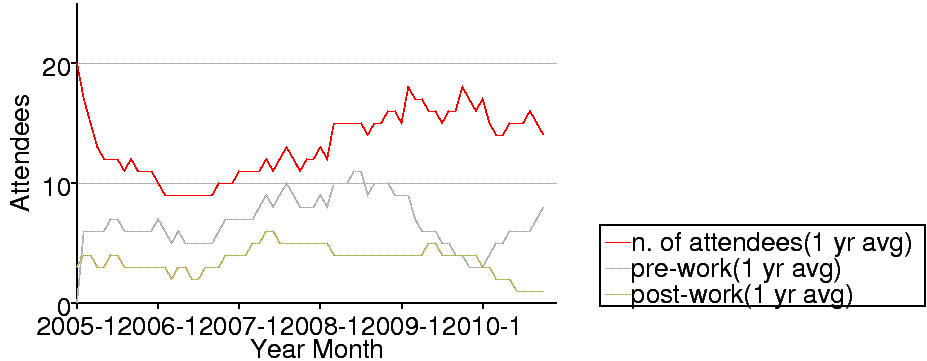
\includegraphics[width=1\hsize]{image201012/memberanalysis/attend.png}\\
 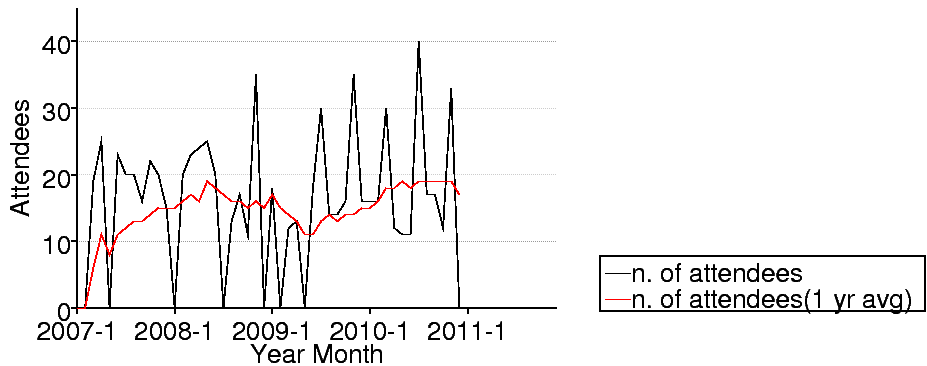
\includegraphics[width=1\hsize]{image201012/memberanalysis/kansai.png}
\end{frame}

\begin{frame}{2010年の成果}

\begin{tabular}{|c|c|c|}
\hline
 & 2009 & 2010 \\
\hline
DDになった人 & 矢吹、谷口、岩松 & やまねひでき \\
NM &  & kiwamu, 上野だいき \\
DM & & kurashiki, kiwamu, uwabami...\\
Debian JP 加入 &  & 1人(山田) \\
\hline
\end{tabular}
 
\end{frame}

\begin{frame}{タイムライン 書き直そう!}

{\scriptsize
\begin{tabular}[t]{|p{4em}|p{4em}|p{9em}|p{7em}|p{6em}|}
\hline
2008 &2009 & 2010 & 2011 & 2012 \\
\hline
%2008
python 3.0
ruby 1.9

wine 1.0, wine64 登場

RoR 2.0 登場で普及に

4コア・64bit のCPUがデスクトップに普及、
Core2Quad 値下げ。

ニコニコ動画1000万ユーザ突破、
初音ミクブームに

地デジ関連のPC製品の普及

勉強会の普及(楽天とか)

公衆無線LAN (wireless gate)

携帯電話の売上が落ちる、
iPhone, Android 登場、
emobile 100円PC抱きあわせ
(eeePC, Dell mini9)
Zaurus販売終了。

Chumby 発売。

サーバの仮想化 ESXi・シンクライアント

MacBook Air 発売、
無線 802.11n が実機に

SystemZ10 発表

世界経済の崩壊(IT投資緊縮財政、職を失う人が増加)

FreeBSD 7 (malloc, ZFS ?)

Debian次世代育成計画始動

Debian Maintainer 制度始動

セキュリティー関連(OpenSSL 事件、DNS事件)

クラウド関連が流行?

Nintendo DSi

&
%2009
政権交代,スパコン事業仕分け,円高

Windows7,Snow Leopard発売

Netwalker発売

MacBookからIEEE1394が消えた。

メモリがDDR3に移行中,メモリ高騰

マジコン販売取り締まり

ラブプラス,OSSを使ったエロゲー登場(OpenCV),AR,セカイカメラ

JLSでLinus来て大騒ぎ

DD,2世誕生

デジタルサイネージ

Google Voice,Wave,Chrome,Chrome OS,Go,日本語入力,徒歩ナビ

CouchDB

Twitter,*なうブーム

Eye-Fi,Kindle2,DS LL,PSP-GO,POKEN

Cell終了のお知らせ

tile window manager boom ?

Lenny リリース

Debian 結婚ブーム

デスクトップ、4コア、8GB

ノートパソコン、2コア、4GB

Linux が標準インストールのPC。(Dell)

SSD の値段と容量がこなれる(まあまあ)
HDDがなくなる?高くなる?(ならず)

SSD特化したFSが出てきた

ipv6 使えるようになってる(来年)

DL禁止法? torrent に逆風?

&
%2010

Toystory 3

デスクトップPC:QuadCore普通。

DDR3 安い、8GB 8000円

ノートパソコン:
NetBookかとおもいきやタブレットPCが普及。

iPhone4、iPad

Willcom再生(Softbankに)

Sun終了

% はやぶさ帰還、あかつき失敗

% NTT vs Softbank 光の道

% 今年も首相交代

自炊ブーム、電子書籍、kindle とか。

kFreeBSD リリースされそう、
zfs がデフォルトで選べる

BtrFSこなかった。ext4 きた。

IS01祭り、Android祭り。

ARM 全盛

クラウド流行

KVS大流行

% Willcom -> Softbank
% SSD
% SIm lock free not yet
% Android だらけ
% Netbook涙目、iPad タブレット盛り上がり
% Cloud!
% iPhone4
% 民主終了、自民は???
% ext4がきた
% kFreeBSDが本当にリリースアーキテクチャになりそう
% Toystory 3 はきた。
% 消費税まだあがっていない
% USB 3.0 なにそれ
% ARM 全盛、Atomあまり普及せず。
% ruby 2.0 なにそれ


&
%2011

デスクトップ終了?
高速化しない。

ノートパソコン:
ChromeOS?
Android?

WebOS終了のお知らせ?

Adobe Flash復活のお知らせ。Silverlight終了のお知らせ(台湾を除く)。

Squeezeリリース。

IPv4割り当ての終了のお知らせ

地上波デジタル移行延長

Btrfsまだ頑張る

Java終了

Open OfficeがOracle Officeに

&
%2012

デスクトップ:終了している。

サーバ:
光インターコネクト?VPS以外はない?

ノートパソコン:Intelじゃないもの(MIPS/ARM)が主流に。

携帯電話:
ガラパゴスの終焉。
LTEが主流になっていない。
Softbankの二年契約が終了、SIM Freeがあたりまえに?

日立と東芝ハードディスク事業を売却統合?

液晶が絶滅。

OracleがBtrfsを終了させる

MySQLがOraSQLに

% Mixi炎上、Facebookが救済、か?

MacBookが新しい基盤に。

\\

\hline
\end{tabular}

}
\end{frame}

\begin{frame}{これをふまえて}
\begin{itemize}
%  \item 1月に新年会と12月の忘年会をする(山本)
%  \item いろんなデバイスの購入計画を立てる(Henrich)
%  \item どんなデバイスがでてもよいようにハック力を鍛えておく(Ar)
%  \item 新しいガジェットを購入していじりたおす会をする(山本)
 \item 新年最初にKinectのネタをやります。(山田)
 \item PS Moveのネタをやる。(岩松)
 \item Squeezeリリースパーティー(Ar)
 \item Mini Debconfをやる(岩松)
 \item SqueezeをふまえてOSCでHands Onをする(やまね)
% \item Sidをいれてみる(山本)
 \item デジタル放送の取り込み(山本)
 \item Debianデジタル放送(岩松)
 \item Debian Pod castやろう(岩松)
 \item 「100台をSqueezeにアップグレードして(吐血)」体験記
 \item OSCでハックラボ、ハックカフェ
 \item 携帯用デバイスにDebianをいれたい。どこまでDebian?
\end{itemize}
\end{frame}

\begin{frame}{2011年どうするか}

\begin{itemize}
 \item こないと何やっているかわからない。Ustream、ブログ、ツイッターに書
       く。
       公式ハッシュタグ(笑)は \#tokyodebian。togetterでまとめる。
       音声認識でtsudaってほしい。
       twitter はフリーではないのでidenti.ca も?
 \item ハックカフェ定期的にする
 \item OSCがある月にも勉強会を開催するか?(運営的にはしんどい?)
 \item Debian勉強会からOSCに全部出てみる。
\end{itemize}

\end{frame}
 
\begin{frame}{2015年の日本}

\begin{itemize}
 \item PC製造:中国系PCメーカーが主導権をにぎる
 \item 世界的にモバイルデバイスが主流になる
 \item 電波通信:NFCのプロトコルがよりひろく使われるようになり、
       NFCのプロバイダーがだれでも提供できるようになる、
       生活にNFCが必須になる
 \item 老人性痴呆症でも使えるPCが登場する
 \item クラウド事業者関連の法制度が整備される
 \item 日本の65歳以上の人口がほげほげ
% 平成19年 人口動態統計の年間推計

\end{itemize}

\end{frame}

\begin{frame}{新年会}

\end{frame}

{\footnotesize
%\begin{prework}{ matsuu }

やったこと・おきたこと
\begin{itemize}
 \item Debian勉強会に参加するようになった。
 \item VPSでDebianを使い始めた。
 \item Debianのパッケージを参考にGentooパッケージを作った。
\end{itemize}
予想・やりたいこと
\begin{itemize}
 \item DebianとGentooは徐々に衰退していき、ALL YOUR DISTRIBUTION ARE
       BELONG TO CHROMEOS.
\end{itemize}
\end{prework}

\begin{prework}{ あらきやすひろ }

予想
\begin{itemize}
 \item 無事リリースされることによるDebian派生ディストロの大崩壊と回帰。
\end{itemize}
やりたいこと
\begin{itemize}
 \item Debianで仕事!
\end{itemize}
\end{prework}

\begin{prework}{ koedoyoshida }

やったこと
\begin{itemize}
 \item ddtssでレビュー(最近お休み中)
 \item 関西KOFでの関西Debianブースのお留守番
 \item 夏冬のイベントでの書籍の頒布
\end{itemize}
おきたこと
 \begin{itemize}
  \item Squeeze freeze
\end{itemize}
予想
\begin{itemize}
 \item  Squeeze release?
\end{itemize}
やりたいこと
\begin{itemize}
 \item 予定は未定
\end{itemize}
\end{prework}

\begin{prework}{ キタハラ }

やったこと
\begin{itemize}
\item 今年は一番何もしていない年ではないだろうか?ネットサーフィン用寝床PCも死んだままだし。
\end{itemize}
やりたいこと
\begin{itemize}
\item 来年はこれを復活し、あと会社にDebianマシンを復活させたいですね。
\end{itemize}
\end{prework}

\begin{prework}{ yamamoto }

やったこと
\begin{itemize}
 \item なんかポチポチと勝手に ppc64 ポートを、マズいラーメン屋の頑固オヤ
       ジのごとく、細く長く続けていた。
\end{itemize}
おきたこと
\begin{itemize}
 \item debian-ports に、sparc64 やら powerpcspe やら armhf やらがいきな
       り現れて、いっきに抜かれて行った。
\end{itemize}
予想
\begin{itemize}
 \item 次は arm64 かな?
\end{itemize}
やりたいこと
\begin{itemize}
 \item 頑固オヤジの迷惑なラーメンを、ひたすら生み出していく。
 \item arm64 ポートに参加できるといいな。
\end{itemize}
\end{prework}

\begin{prework}{ 本庄 }

やったこと
\begin{itemize}
\item 温泉行きました。
\end{itemize}
やりたいこと
\begin{itemize}
\item また行きたいです。
\end{itemize}
\end{prework}

\begin{prework}{ yyuu }

私事ではありますが、2009 年くらいから仕事で Debian を使えるようになりま
 した。2010 年はその環境の整備に費やしているうちにあっという間に過ぎてし
 まいました。

やったこと
\begin{itemize}
 \item lenny のシステムを 100 台以上の単位で扱うことができた
 \item 自分で個人的な apt のレポジトリを作って運用できるようになった
\end{itemize}
おきたこと
\begin{itemize}
 \item 特に思いつきませんでした...
\end{itemize}

予想
 \begin{itemize}
  \item squeeze がリリースされる (2010年?)
 \end{itemize}
やりたいこと
\begin{itemize}
 \item 一部の既存ホストを lenny から squeeze へ移行したい
 \item 新興プロジェクトの Debian パッケージ化にできるだけコミットしてい
       きたい。今年は Apache Thrift などにパッチを提供できたが、今後はも
       う少し手を広げたい
\end{itemize}
\end{prework}

\begin{prework}{ 野島 貴英 }

やったこと
\begin{itemize}
 \item debian-sidのKVM上でOpensolarisを稼働させた事。
 \item debian-sidの様々なソースコードいっぱい読んだこと。
       \footnote{\url{http://d.hatena.ne.jp/nozzy123nozzy/}}
\end{itemize}
予想
\begin{itemize}
\item いわゆる携帯型tabletPC等へdebian-sidを搭載するHackがそこいら中で起きる。
\end{itemize}
やりたいこと
\begin{itemize}
 \item Contribution \& Hack!Hack!Hack!(ソフトもハードも)
\end{itemize}
\end{prework}

\begin{prework}{ henrich }

やったこと
\begin{itemize}
 \item 5月: NMプロセスを進めてDDになった
 \item 7月: スイスからDebian傘買ってみた :)
 \item 8月: Debconf に参加した
 \item パッケージのアップデートを大体継続できた
 \item その他国内のイベントに参加した
 \item RC バグ潰しに参加した
 \item 多少ではあるが翻訳作業に参加した
 \item 手が付いていないことは以下
       \begin{itemize}
	\item netbeans のパッケージ
	\item eclipse-l10n のパッケージ(ソースを見つけられない…)
	\item Knoppix-Math を Debian ベースに誘う
	\item lenny インストール記事を JP ページに載せる
       \end{itemize}
\end{itemize}
やりたいこと
\begin{itemize}
 \item 開発者リファレンス訳の完了
 \item 初歩のプログラミングができるように(pythonあたり)
 \item debconf で何かしらの成果を出せるように事前準備
 \item l10n をもっと進められるようにもっとステップと成果を明確にしたい
\end{itemize}
\end{prework}

\begin{prework}{ 岩松 信洋 }

やったこと
\begin{itemize}
 \item 組み込み関係のサポート。
 \item SH4のemdebianサポート。
 \item Macbook 関係のサポート。
 \item DDになってからの始めてのリリース作業。
 \item Debconf への参加
\end{itemize}
おきたこと
\begin{itemize}
 \item Non-packaging contributors
 \item backports が正式サービスになった。 
 \item Squeeze フリーズ
 \item Miniconf が多く行われた。
 \item fjp の急逝
\end{itemize}
予想
\begin{itemize}
 \item Debian では SH4 unstable 入り
 \item 4G ネットワークがじわじわと浸透
 \item Android を使ったタブレットデバイス祭り
\end{itemize}
やりたいこと
\begin{itemize}
 \item web 系の開発
 \item 関数型言語の習得
\end{itemize}
\end{prework}

\begin{prework}{ 野首 }

2010年はほとんど何もしませんでした...
さすがにsqueezeは2011年にはリリースされていると思いたい。
\end{prework}

\begin{prework}{ まえだこうへい }

やったこと
\begin{itemize}
 \item Debian勉強会の運営(いつもどおり)
 \item 山田さんのJPへの勧誘・加入(よくやった)
 \item 他の勉強会での勧誘(Webアプリ開発者に交友関係は増えたがDebianへの
       直接的な成果はなし)
\end{itemize}
おきたこと(予想?)
\begin{itemize}
 \item SqueezeにはCouchDB 1.0.1が入らなさそう。
\end{itemize}
やりたいこと
\begin{itemize}
 \item いろいろpendingなものを再開する。
\end{itemize}
\end{prework}

\begin{prework}{ 上川純一 }

やったこと
\begin{itemize}
 \item 子供がうまれた、Debian活動レベルが低下した。
 \item 携帯電話はAndroid携帯電話がメインになって、パソコンをあまり起動し
       なくなった。
 \item 勉強会にくるようなメンバーで、Smart Phone (iPhone or Android)をもっ
       ていない人に出会わなくなってきた。
\end{itemize}
予想
\begin{itemize}
 \item さらなるスマートフォンとタブレットの普及とそれに伴うより自由で便
       利な環境への渇望。
 \item Debianとしてはその環境との相互運用性の向上と、そのデバイス自体で
       動くシステムとしてのすすみかたが二つ考えられる。
\end{itemize}
やりたいこと
\begin{itemize}
 \item 相互運用性は少なくとも向上したいと考えている。
\end{itemize}
\end{prework}


}

\section{DWN quiz}
\begin{frame}{Debian 常識クイズ}

Debian の常識、もちろん知ってますよね?
知らないなんて恥ずかしくて、知らないとは言えないあんなことやこんなこと、
みんなで確認してみましょう。

今回の出題範囲は\url{debian-devel-announce@lists.debian.org} に投稿された
内容とDebian Project Newsからです。

\end{frame}

\subsection{問題}
%; whizzy-master ../debianmeetingresume200906.tex
% $B0J>e$N@_Dj$r$7$F$$$k$?$a!"$3$N%U%!%$%k$G(B M-x whizzytex $B$9$k$H!"(Bwhizzytex$B$,MxMQ$G$-$^$9!#(B
%
% $B$A$J$_$K!"%/%$%:$OJL%V%i%s%A$G:n@.$7!"$N$A$K%^!<%8$7$^$9!#5U$K%^!<%8$7(B
% $B$J$$$h$&$K$7$^$7$g$&!#(B
% (shell-command "git checkout quiz-prepare")

\santaku
{DACA $B$C$F$J$s$G$9$+(B?}
{Debian Admin Coaching Association}
{Debian $B$r;H$&$H(B (A)$B$"$N;R$H(B (C)$B%/%j%9%^%9$K(B (A)$B%"%l$,$G$-$k$+$b$7$l$J$$(B}
{Debian's Automated Code Analysi project}
{C}

\santaku
{DebConf11 $B$O$$$D3+:E$5$l$k$G$7$g$&(B}
{2011/6/24 - 30}
{2011/7/24 - 30}
{2011/8/24 - 30}
{B}

\santaku
{squeeze $B$N(B Linux $B%+!<%M%k$O0lL#0c$$$^$9!#2?$,0c$&$G$7$g$&!#(B}
{non-free firmware $B$rGS=|$7$?(B}
{Tux $B$/$s$rGS=|$7$?(B}
{$B0l$D$N%+!<%M%k%$%a!<%8$G(BkFreeBSD$B$H(BLinux$B$rDs6!$7$^$9(B}
{A}

\santaku
{2010/12/17 $B$N;~E@$G(BRC$B%O%0$O$$$/$D$"$k$G$7$g$&!#(B}
{3} 
{83}
{183}
{C}

\santaku
{New Maintianer $B%U%m%s%H%G%9%/$KDI2C$5$l$?%a%s%P!<$O!)(B}
{Xavier Oswald}
{Enrico Zini}
{Kenshi Muto}
{A}




\emtext{2010年のDebian勉強会を振り返って}

\emtext{CACertの準備に必要なもの}

\emtext{俺のlibsaneが火をふくぜ}

\emtext{Debian Miniconf 企画}

\emtext{2011 年を想像する}

\end{document}

;;; Local Variables: ***
;;; outline-regexp: "\\([ 	]*\\\\\\(documentstyle\\|documentclass\\|emtext\\|section\\|begin{frame}\\)\\*?[ 	]*[[{]\\|[]+\\)" ***
;;; End: ***
